\chapter{User-modelled ambient feedback for self-regulation}

\vfill
A fundamental objective of human-computer interaction research is to make systems that are seamlessly integrated into daily life activities. Hence, the challenge for technology enhanced-learning research is not only to make in-formation available to people at any time, at any place, and in any form, but specifically to say the �right� thing at the �right� time in the �right� way. On the other hand, the proliferation of sensor technology is facilitating the scaffolding and customization of smart learning environments. This manuscript presents an ecology of resources comprising NFC, BLE and Arduino technology, orchestrated in the context of a learning environment to provide smoothly integrated feedback via ambient displays. This ecology is proposed as a suitable solution for self-regulation, providing support for setting learning goals, setting aside time to learn, tracking study time and monitoring the progress. Herby, the ecology is described and intriguing research questions are introduced.
\vspace{3em}

This chapter has been submitted as: 
Tabuenca, B., B\"orner, D., Kalz, M., \& Specht, M. (2015). User-modelled ambient feedback for self-regulation
. Demo paper

\clearpage

\section{Introduction}
Providing in-context support and feedback is key to identify the best learning moments and self-organize the learning day. Lifelong learning implies setting aside regular time for learning during the day as well as combining learning activities with daily life activities (i.e. family, work, leisure). Nevertheless, daily contingencies and their varying priorities make specially challenging to provide technological support for lifelong learners in the task to set realistic goals, set aside daily time to learn, track the time devoted to learn, and monitor learning progress. In previous research, we investigated different ways to provide feedback services fostering the competence of �learning to learn�, using SMSs (see chapter 8) and mobile chart visualizations (see chapter 9) as channels to provide guidance from the teacher (external feedback). The differentiation among external and internal feedback is crucial if one investigates the effects of feedback on the basis of recent instructional models viewing the process of knowledge acquisition as a self-regulated learning process \citep{Narciss2007}. Hence, hereby we present a smart learning ecology in which lifelong learners are able to customize internal feedback based on their own occasional learning priorities and contingencies.

\section{Smart ecology of resources for time management}
\citep{Candy1991} summarized four components of self-directed lifelong learning: self-monitoring, self-awareness, self-management and meta-learning. The challenge in an information-rich world is not only to make information available at any time, at any place, and in any form, but specifically to say the �right� thing at the �right� time in the �right� way \citep{Fischer2001}. This ecology provides self-regulated support for lifelong learners tracking time devoted to learn, orchestrating sensor technology, and modelling ambient feedback. 

The NFC-LearnTracker \citep{Tabuenca2014f} is an open source mobile application developed for NFC-enabled devices that features learning analytics of time devoted to learn based on the timestamps recorded every time the user starts (check-in) and stops (check-out) a self-defined learning goal. The evaluation of the NFC-LearnTracker \citep{TabuencaLT2014b} concluded that it is a useful tool to set and adjust mini-goals, to foster awareness on preferred learning environments, and to integrate learning in daily activities.

\begin{center}
\begin{figure}[ht]
\centering
	\subfloat[Feedback Cube \ BLE-beacon]{
		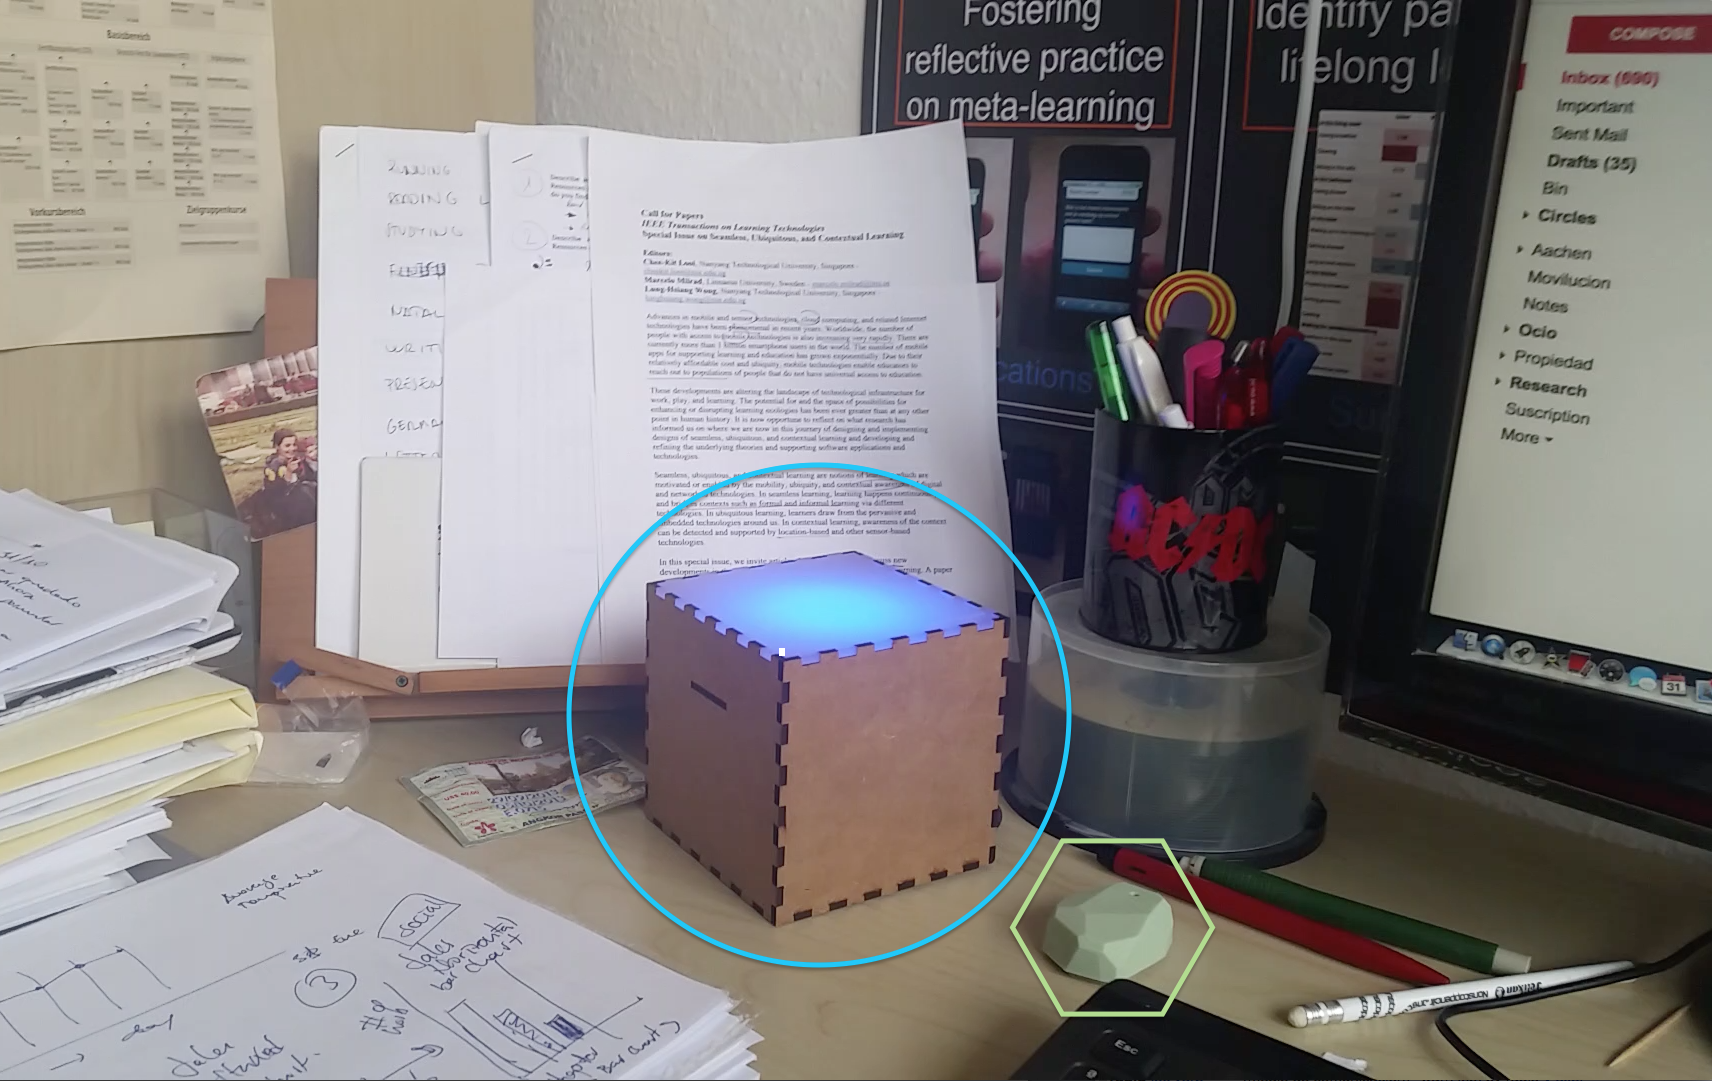
\includegraphics[height=0.3\linewidth]{img/nfceco_fig1}
		\label{fig:nfceco_1}
	}
	\subfloat[NFC-tags bound to learning activities]{
		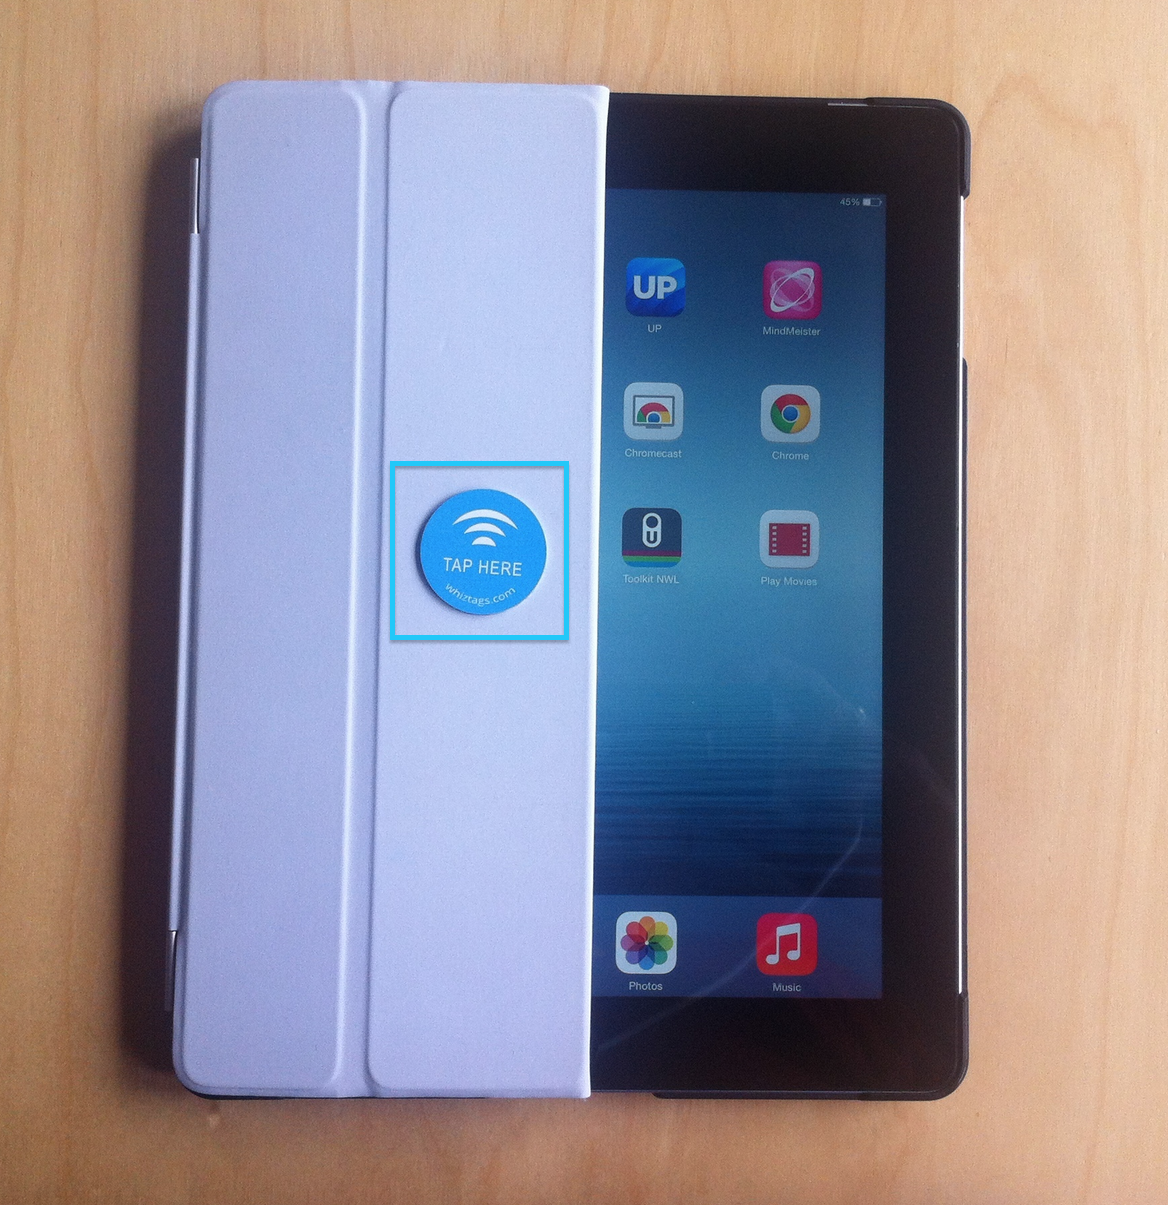
\includegraphics[height=0.3\linewidth]{img/nfceco_fig2}
		\label{fig:nfceco_2}
	}	
	\subfloat[NFC-LearnTracker's learning analytics]{
		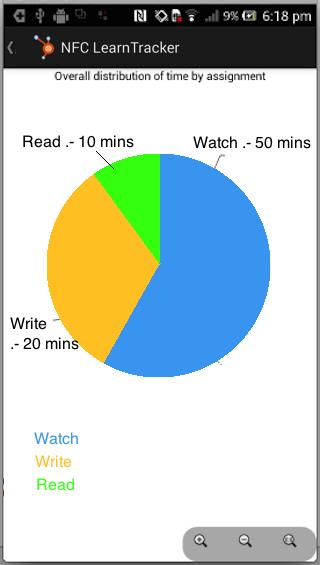
\includegraphics[height=0.3\linewidth]{img/nfceco_fig3}
		\label{fig:nfceco_3}
	}
      \caption{Ecology of resources for time management}	
\end{figure}
\end{center}

The NFC-LearnTracker interprets the information provided by the following sensors:
\begin{itemize}
\item NFC tags (fig. \ref{fig:nfceco_2}. See blue squared). As illustrated in figure \ref{fig:nfceco_3}, an overall learning goal (i.e. learn Dutch) comprises a set of sub-goals (watch videos; write texts: read news) that are assigned a coloured tag (blue; orange; green), an estimated daily time in minutes (50; 20; 10), and a deadline date to accomplish each sub-goal (31st December of 2015).
\item Bluetooth Low Energy (BLE) beacons (fig. \ref{fig:nfceco_1}. See green hexagon). BLE-beacons are being novelty used to provide proximity-adapted feedback in the field of shop-ping , access control, and home entertainment. Herby, we use BLE-beacons to monitor student�s progress when he approaches or moves away from the beacon (i.e. desktop at home; office at workplace).
\end{itemize}
The Feedback Cube \citep{Borner2015} (fig. \ref{fig:nfceco_1}) is an ambient learning display \citep{Borner2013} built-on an Arduino microcontroller that provides visual and audio feedback (fig.\ref{fig:nfceco_3}). The used LEDs are capable of displaying the full RGB colour space with 16777216 colours at 256 bright-ness levels (fig. \ref{fig:nfceco_5}). All 16 RGB LEDs on the ring can be controlled individually, which allows programming various visual patterns (fig. \ref{fig:nfceco_6} matches pie chart in fig. \ref{fig:nfceco_3}) and effects, such as fading, blinking, or colour transitions. The used mini speaker can reproduce programmatically created audio patterns and effects, such as playing single tones, complex melodies, or even encoded audio files.

\begin{center}
\begin{figure}[ht]
\centering
	\subfloat[Sound and color]{
		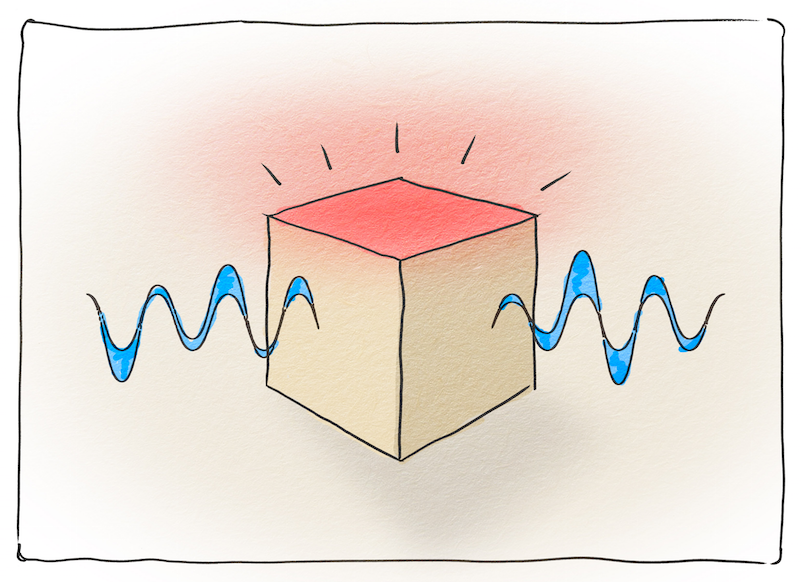
\includegraphics[width=0.3\linewidth]{img/nfceco_fig4}
		\label{fig:nfceco_4}
	}
	\subfloat[Rainbow]{
		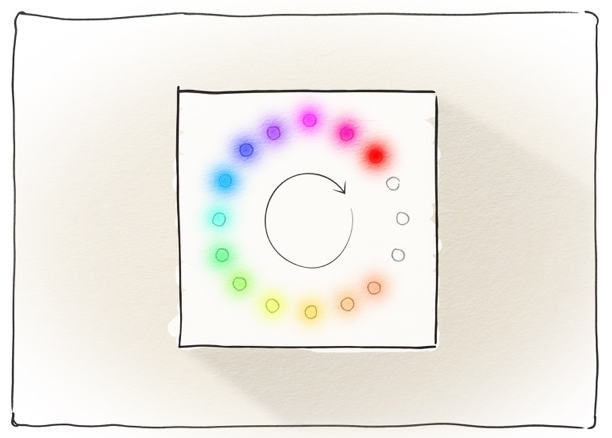
\includegraphics[width=0.3\linewidth]{img/nfceco_fig5}
		\label{fig:nfceco_5}
	}	
	\subfloat[Pie chart]{
		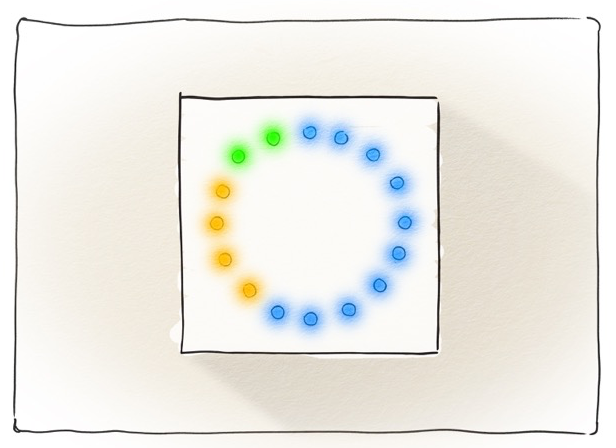
\includegraphics[width=0.3\linewidth]{img/nfceco_fig6}
		\label{fig:nfceco_6}
	}	
      \caption{Feedback Cube's effects}
\end{figure}
\end{center}

\section{Mapping events and feedback}

The NFC-LearnTracker lets the user configure which feedback signal fits better each one of the events listed below. Herby we present the events supported and their default set-up:

\begin{table}[h]
  \centering
  \footnotesize
  
\begin{tabular}{|l|l|l|}
\hline
\multicolumn{1}{|c|}{\textbf{Event}}                                                                         & \multicolumn{1}{c|}{\textbf{Action}}                                                                                  & \multicolumn{1}{c|}{\textbf{Feedback}}                                                                                                                  \\ \hline
On approach                                                                                                  & \begin{tabular}[c]{@{}l@{}}The user moves closer\\ to the BLE beacon\end{tabular}                                     & \begin{tabular}[c]{@{}l@{}}Summarize! The cube lights a pie\\ chart indicating the distribution of\\ time for pending tasks (fig.6)\end{tabular}        \\ \hline
On check-in                                                                                                  & \begin{tabular}[c]{@{}l@{}}The user taps on the\\ NFC tag every time a\\ learning activity is\\ started.\end{tabular} & \begin{tabular}[c]{@{}l@{}}Start! The cube lights the blue colour\\ (fig.1) to indicate your are working\\ on the blue learning goal\end{tabular}       \\ \hline
On check-out                                                                                                 & \begin{tabular}[c]{@{}l@{}}The user taps on the\\ NFC tag to stop a \\ learning activity.\end{tabular}                & \begin{tabular}[c]{@{}l@{}}Stop! The cube switches off the\\ existing light\end{tabular}                                                                \\ \hline
\begin{tabular}[c]{@{}l@{}}X minutes before expiring\\ the estimated time for a\\ goal in a day\end{tabular} & \begin{tabular}[c]{@{}l@{}}X minutes before \\ time expires\end{tabular}                                              & \begin{tabular}[c]{@{}l@{}}Time to wrap up! The cube slowly\\ fades X� times to gently advice that\\ time will expire in X minutes.\end{tabular}        \\ \hline
\begin{tabular}[c]{@{}l@{}}On expiry estimated time\\ for a goal in a day\end{tabular}                       & Time expired                                                                                                          & \begin{tabular}[c]{@{}l@{}}Time just expired! The cube beeps\\ once providing a more intrusive\\ notification\end{tabular}                              \\ \hline
\begin{tabular}[c]{@{}l@{}}Y minutes after expiring \\ the estimated time for a\\ goal in a day\end{tabular} & \begin{tabular}[c]{@{}l@{}}Y minutes after \\ expiring\end{tabular}                                                   & \begin{tabular}[c]{@{}l@{}}Overworking! The cube fades faster \\ Y� times warning that you exceeded\\ Y minutes your scheduled time.\end{tabular}       \\ \hline
\begin{tabular}[c]{@{}l@{}}On accomplishment of \\ all goals in a day\end{tabular}                           & \begin{tabular}[c]{@{}l@{}}On check-out \\ the last goal\end{tabular}                                                 & \begin{tabular}[c]{@{}l@{}}All daily goals accomplished! The\\ cube lights a rainbow to congratulate\\ the user\end{tabular}                            \\ \hline
\begin{tabular}[c]{@{}l@{}}On accomplishment of\\ one-goal deadline date\end{tabular}                        & \begin{tabular}[c]{@{}l@{}}Scheduled date \\ to finishone goal\end{tabular}                                           & \begin{tabular}[c]{@{}l@{}}Learning goal accomplished! The\\ cube plays a melody indicating the\\ goal is finished\end{tabular}                         \\ \hline
\begin{tabular}[c]{@{}l@{}}On accomplishment \\ of all-goals deadline \\ date\end{tabular}                   & \begin{tabular}[c]{@{}l@{}}Scheduled date \\ to finish\\ the last goal\end{tabular}                                   & \begin{tabular}[c]{@{}l@{}}All goals accomplished! The cube\\ lights a rotating rainbow to congratu-\\ late the user\end{tabular}                       \\ \hline
On move away                                                                                                 & \begin{tabular}[c]{@{}l@{}}The user moves away\\ from the BLE beacon\end{tabular}                                     & \begin{tabular}[c]{@{}l@{}}Summarize! The cube beeps Z� times\\ summarizing pending study time\\ (e.g. 30 minutes pending beeps 3\\ times)\end{tabular} \\ \hline
\end{tabular}
\end{table}

In further research, the quality of the learning analytics via mobile visualizations and ambient displays will be contrasted and evaluated \citep{Scheffel2014}. Additionally, we will explore to which extent internal feedback services improve self-regulation.
